% Present the findings of your research. Provide a detailed 
% analysis of the performance of the various algorithms used 
% for weather prediction, including their accuracy, precision, 
% and recall rates.

% The results section of your thesis presents the findings of 
% your study. It should provide a clear and concise summary of 
% the data collected and analyzed, along with any statistical 
% tests or other methods used to analyze the data. Here are some 
% important elements to consider including in your results section:

% Overall, the results section of your thesis should provide a 
% clear and concise summary of your findings, along with any statistical 
% tests or other methods used to analyze the data. It should also provide 
% an interpretation of your findings and relate them back to your research 
% questions or hypotheses.
\section{Wyniki}

% Descriptive statistics: Provide descriptive statistics that 
% summarize the main characteristics of your data, such as means, 
% standard deviations, and frequency distributions.
\subsection{Statystyki}

Jak widać na rysunku \ref{mse}, w przypadku każdego algorytmu nastąpił
spadek dokładności względem danych testowych. W przypadku modelu KNN oraz
regresji gaussowskiej znikomy błąd na danych treningowych wynika z faktu, 
że obydwa modele bazują na uczeniu na przykładach i ich ewaluacja na 
danych treningowych jest niemiarodajna. 

\begin{figure}[H]
    \centering
    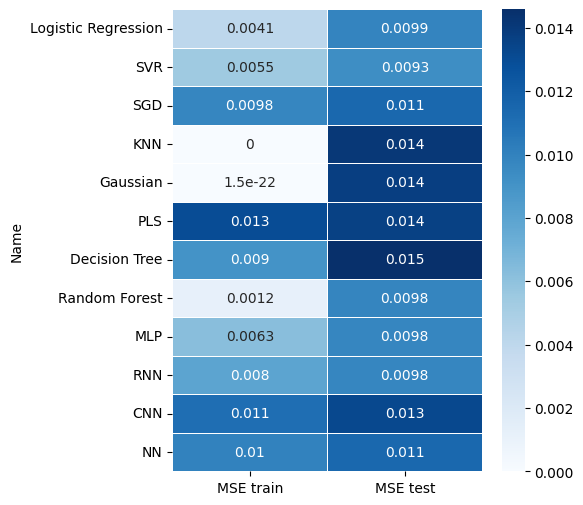
\includegraphics[width=\textwidth]{images/mse.png}
    \caption{Błąd średniokwadratowy dla stworzonych modeli}
    \label{mse}
\end{figure}

Las losowy okazuję się algorytmem, który jest w stanie bardzo dobrze 
dopasować się do danych treningowych razem z zachowaniem ogólności dla 
reszty danych, osiągając dobre wyniki na zbiorze testowym. Z kolei RNN, NN
SVR osiągają zbliżone wartości zarówno dla zbioru treningowego, jak i testowego.

\begin{figure}[H]
    \centering
    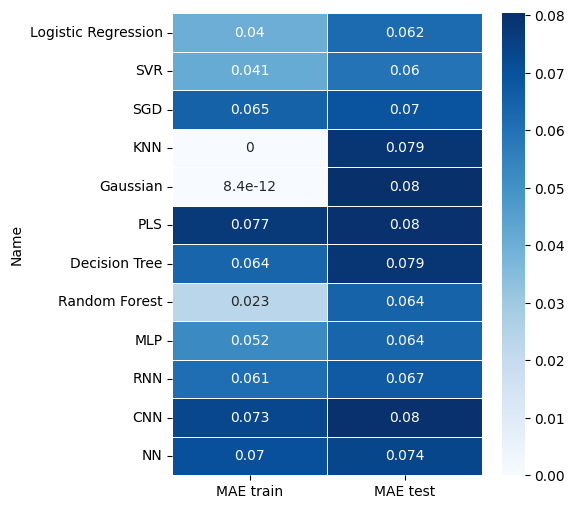
\includegraphics[width=\textwidth]{images/mae.png}
    \caption{Średni błąd absolutny dla stworzonych modeli}
    \label{mae}
\end{figure}

Wartości błędu absolutnego osiągają większe wartości od MSE. Co więcej,
rozbieżność między błędem dla zbioru treningowego i testowego
przy użyciu metryki MAE staje się mniejsza. Ogólna dystrybucja błędu 
względem modeli zdaje się podobna.

\begin{figure}[H]
    \centering
    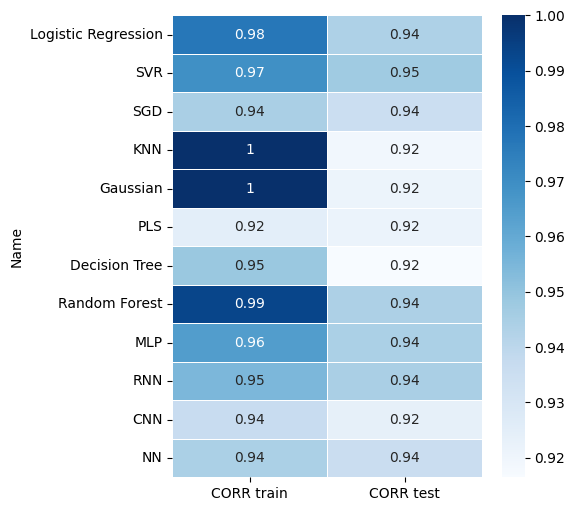
\includegraphics[width=\textwidth]{images/corr.png}
    \caption{Współczynnik korelacji dla stworzonych modeli}
    \label{corr}
\end{figure}

Dla wszystkich modeli współczynnik korelacji pomiędzy wartościami rzeczywistymi 
a przewidzianymi jest na poziomie przekraczającym 0,9. Wskazuje to na dobre dopasowanie
modeli do przewidzianych danych, chociaż warto wskazać, że współczynnik
autokorelacji dla wielu parametrów pozostawał na poziomie powyżej 0,8 dla wartości
opóźnienia przekraczających parę godzin.

\begin{figure}[H]
    \centering
    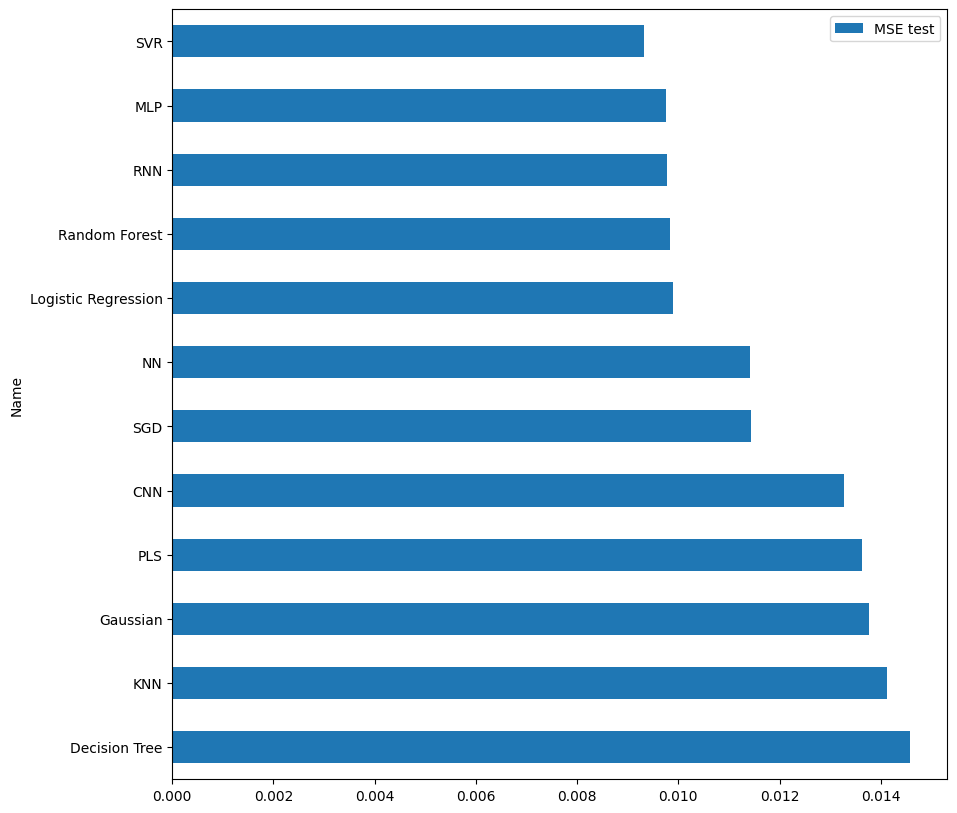
\includegraphics[width=\textwidth]{images/mse_ranking.png}
    \caption{Ranking stworzonych modeli ze względu na błąd średniokwadratowy}
    \label{mse-ranking}
\end{figure}

Na wykresie \ref{mse-ranking} widać stworzony ranking ze względu na wartość MSE.
Najlepszymi algorytmami pod tym względem okazały się SVR, MLP i RNN. Rozbieżność 
pomiędzy najlepszym modelem a najgorszym wynosiła 0,0057. Algorytmami 
osiągającymi najgorsze wyniki był KNN i drzewo decyzyjne.

Można przeprowadzić podobną analizę ze względu na MAE, co zostało pokazane na 
rysunku \ref{mae-ranking}. W tym przypadku o wiele lepsze wyniki 
otrzymała regresja logistyczna i las losowy, które znajdują się wśród najlepiej 
ocenionych algorytmów.

\begin{figure}[H]
    \centering
    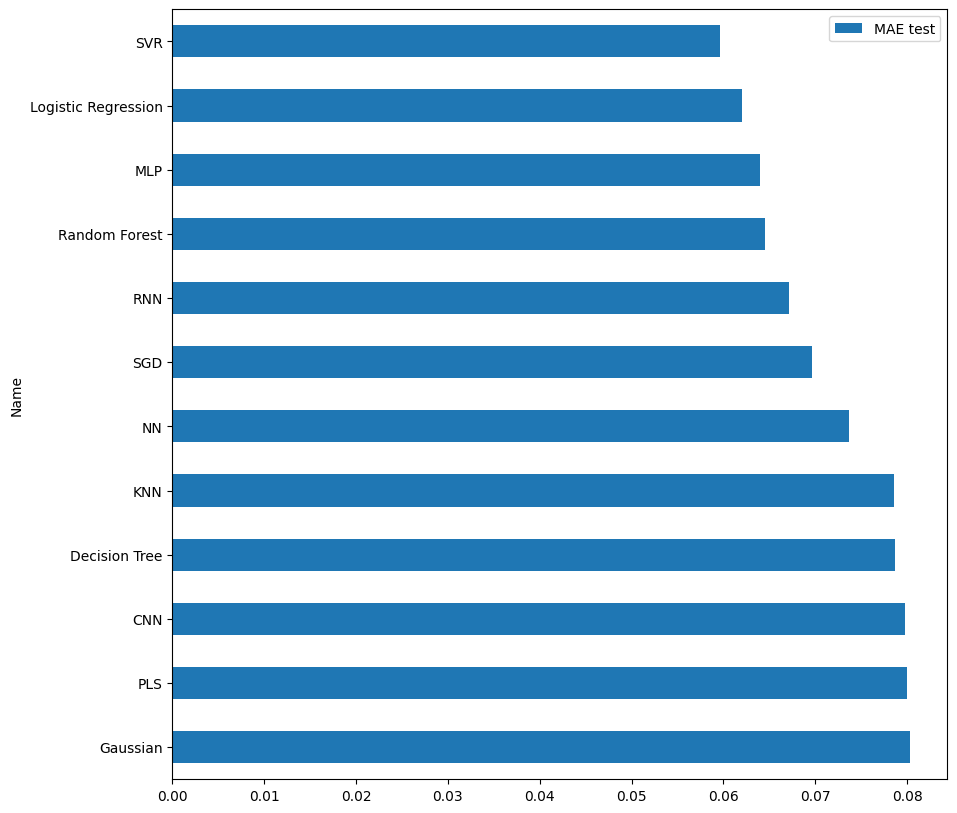
\includegraphics[width=\textwidth]{images/mae_ranking.png}
    \caption{Ranking stworzonych modeli ze względu na średni błąd absolutny}
    \label{mae-ranking}
\end{figure}

Analiza ze względu na korelację pokazuje bardzo zbliżone wartości dla wszystkich 
modeli, a kolejność algorytmów w pokazanym rankingu \ref{corr-ranking} jest 
bardzo podobna do tej ze względu na błąd średniokwadratowy \ref{mse-ranking}.

\begin{figure}[H]
    \centering
    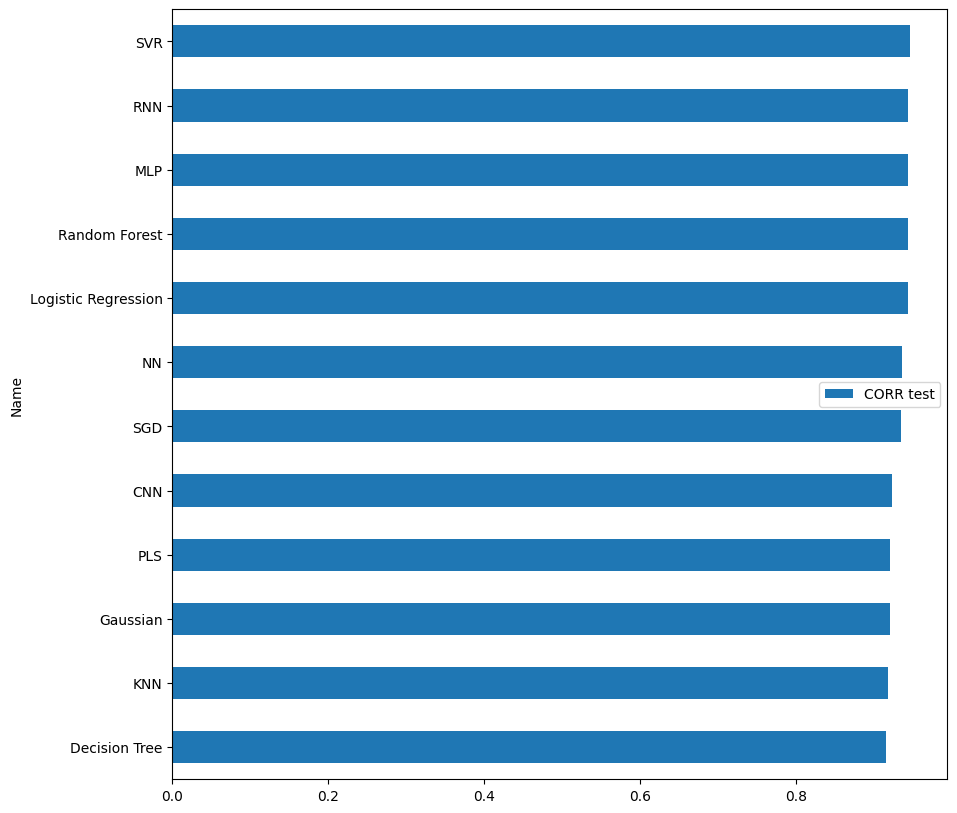
\includegraphics[width=\textwidth]{images/corr_ranking.png}
    \caption{Ranking stworzonych modeli ze względu na wartość korelacji}
    \label{corr-ranking}
\end{figure}

W celu dalszego przybliżenia zachowania poszczególnych modeli, stworzone zostały
zestawienia prawdziwych przebiegów czasowych oraz tych wygenerowanych przez algorytmy
uczenia maszynowego. Chociaż zaprezentowane metryki dają wstępne zrozumienie
stopnia dopasowania modeli oraz ich dokładności, to analiza graficzna jest kluczowa
do zrozumienia, jakie zjawiska są dobrze prognozowane, a jakie stwarzają problemy.
Przedstawione przebiegi prezentują tygodniowe przebiegi złożone z siedmiu 
dwudziestoczterogodzinnych prognoz.

\pagebreak

Jednym z najlepiej ocenianych algorytmów była regresja wektorów wspierających.
W tym przypadku widzimy dobre zachowanie względem przebiegów cyklicznych, takich jak
promieniowanie słoneczne czy odparowanie. Pod względem promieniowania termicznego
widoczne jest dobre odwzorowanie wartości średniej szeregu czasowego, lecz problem
z dopasowaniem do indywidualnych skoków w wartościach.

Nagły skok w wartości opadów został zupełnie pominięty w prognozie i wskazuje 
na problemy z przewidywaniem nagłych zdarzeń o dużej amplitudzie. 

Zarówno wartości prędkości wiatru, jak i temperatury zostały wiernie odwzorowane
przez stworzony model, a na poniższych wykresach widać jak linie prognozowanych wartości
podążają za wartościami przewidywanymi. W przypadku ciśnienia atmosferycznego,
po nagłym spadku model był w stanie dopasować się ponownie do danych pomiarowych
i dalej podążać za utworzonym trendem.

\begin{figure}[H]
    \centering
    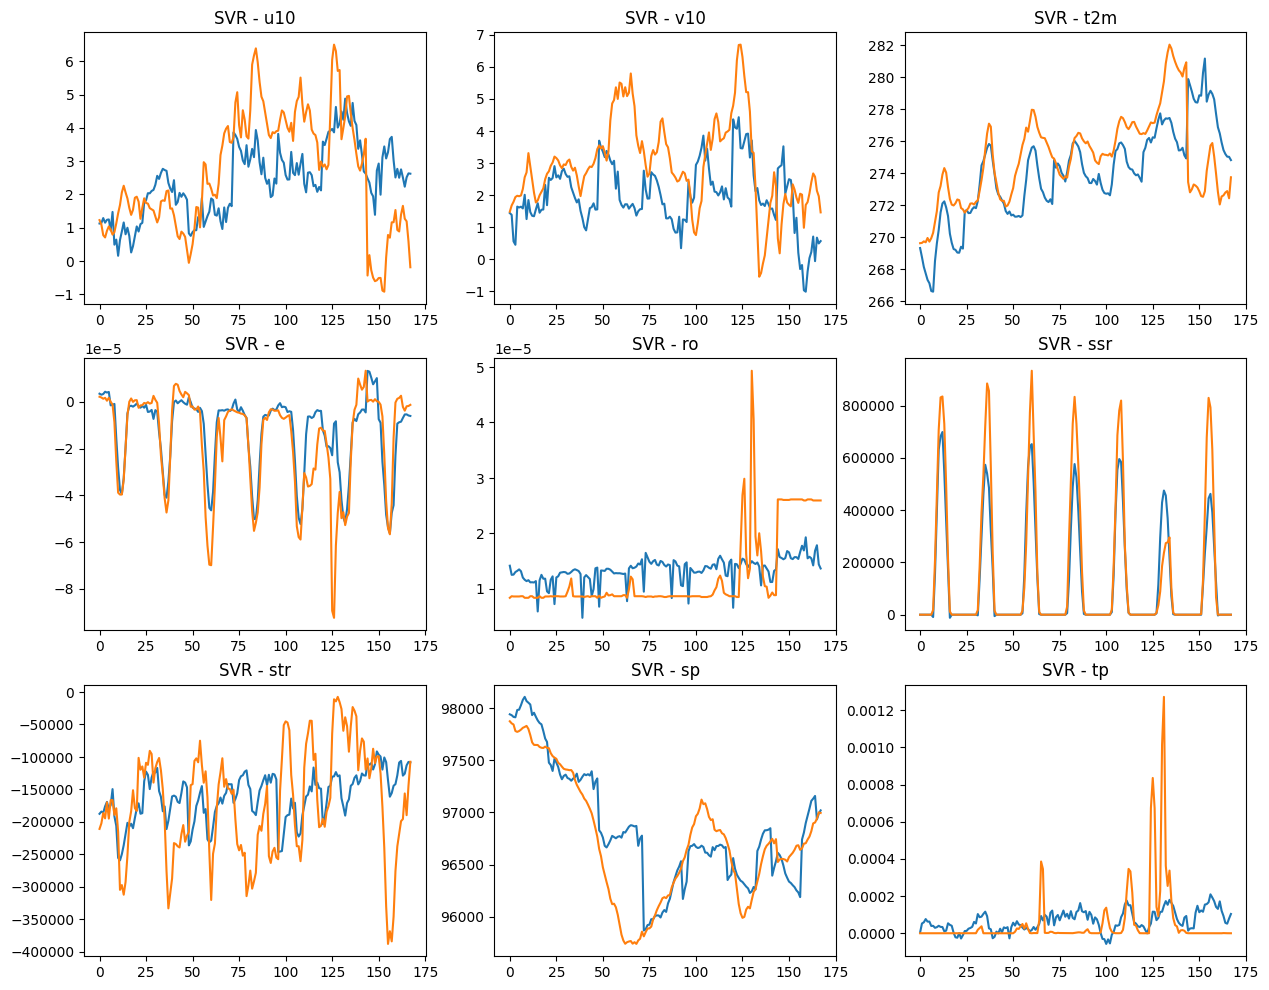
\includegraphics[width=\textwidth]{images/SVR_week.png}
    \caption{Przebiegi czasowe dla algorytmu SVR. Na żółto pokazane zostały dane 
    rzeczywiste, na niebiesko predykcje wygenerowane przez model}
    \label{svr-week}
\end{figure}

Dla perceptronu wielowarstwowego widać dużo większą wariancję w wyjściu modelu 
w zakresie krótkoterminowym. Duże wahania są szczególne widoczne dla wartości odpływów.
Bardzo możliwe, że charakterystyka oscylacyjna danych wejściowych wprowadza znaczną
ilość zakłuceń, a zbyt prosta architektura sieci nie zapewnia możliwości odfiltrowania 
szumów. 

\begin{figure}[H]
    \centering
    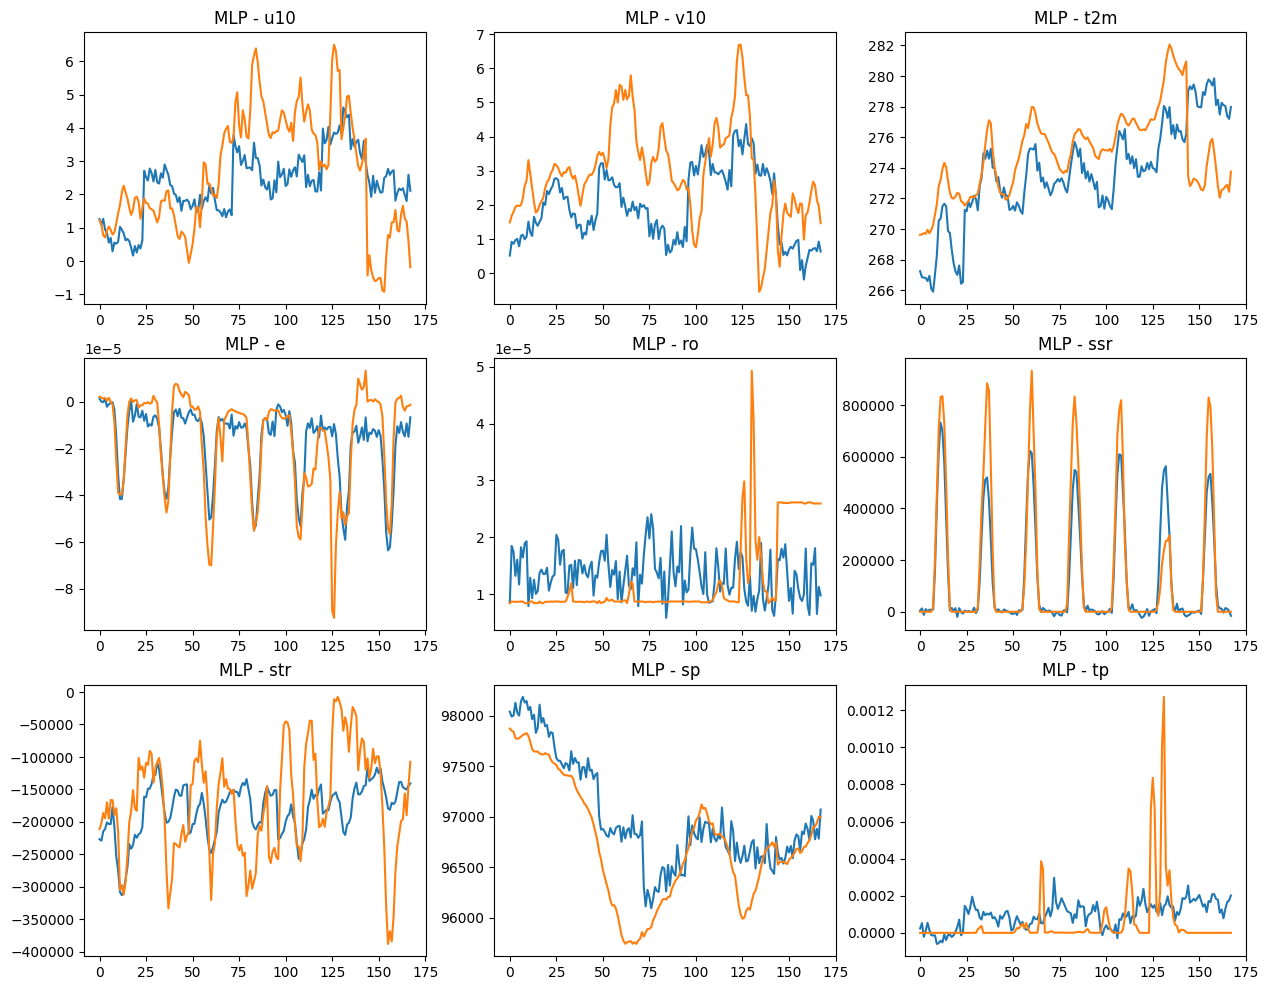
\includegraphics[width=\textwidth]{images/MLP_week.png}
    \caption{Przebiegi czasowe dla algorytmu MLP. Na żółto pokazane zostały dane 
    rzeczywiste, na niebiesko predykcje wygenerowane przez model}
    \label{mlp-week}
\end{figure}

Rekurencyjna architektura sieci neuronowych RNN prezentuje podobne zachowanie 
generując dane wyjściowe z dużymi wahaniami. Wyniki dla tego modelu zostały zaprezentowane na rysunku \ref{rnn-week}

\begin{figure}[H]
    \centering
    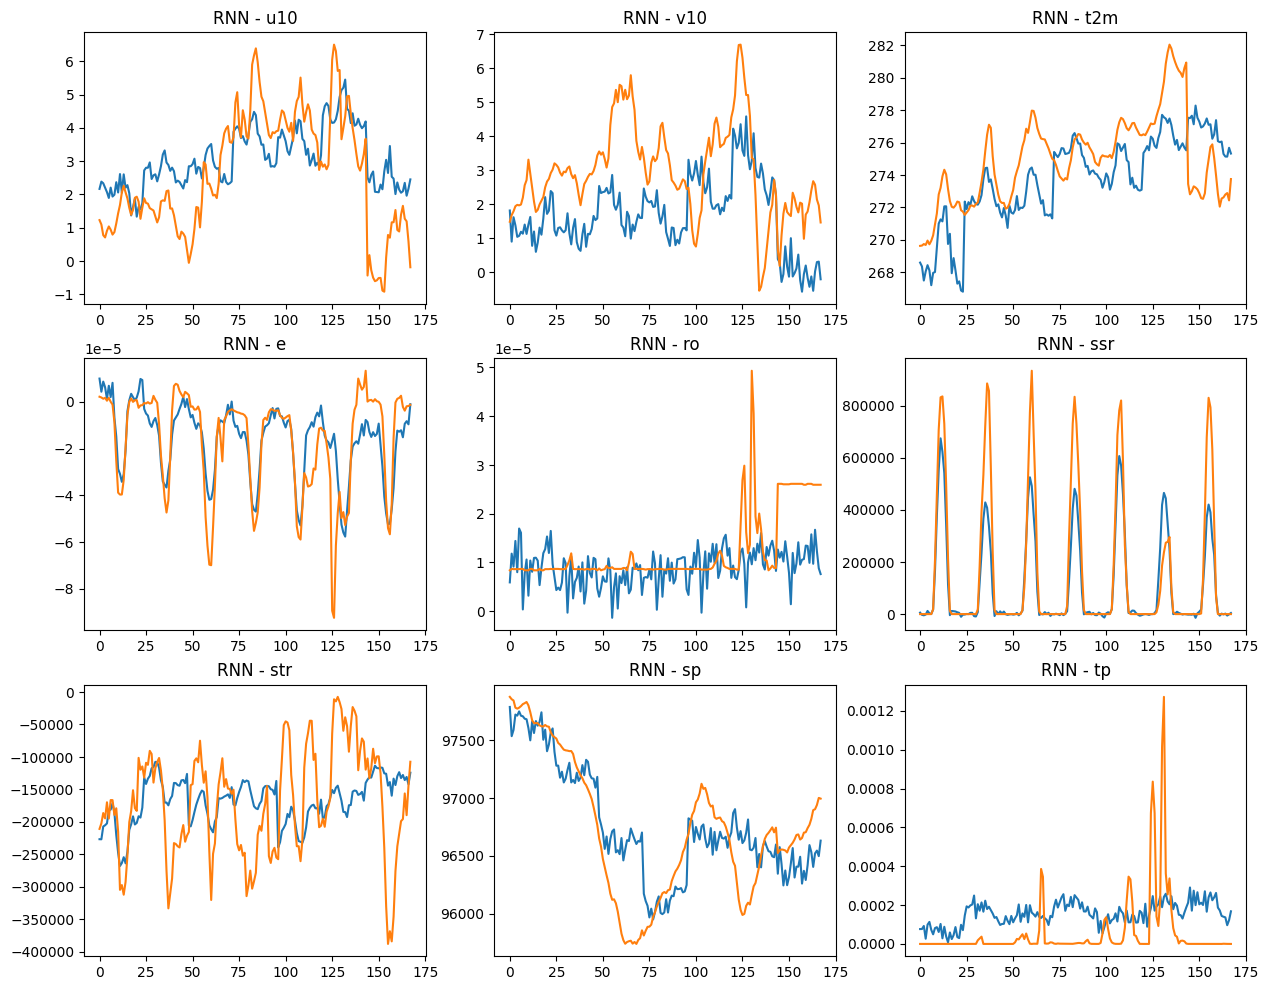
\includegraphics[width=\textwidth]{images/rnn_week.png}
    \caption{Przebiegi czasowe dla algorytmu RNN. Na żółto pokazane zostały dane 
    rzeczywiste, na niebiesko predykcje wygenerowane przez model}
    \label{rnn-week}
\end{figure}

W przypadku lasu losowego, widać duże przesunięcie dla linii odpływów wody. Stworzone prognozy zdecydowanie
przeceniają wartości rzeczywiste, co może być spowodowane pojedynczymi zdarzeniami w zbiorze treningowym o
dużej amplitudzie, które mogły zaburzyć proces uczenia modelu.

Można też zauważyć widoczne wahania o charakterze dwudziestoczterogodzinnym w wartościach 
prędkości wiatru i temperatury, które niekoniecznie odnajdują odzwierciedlenie w danych rzeczywistych.

\begin{figure}[H]
    \centering
    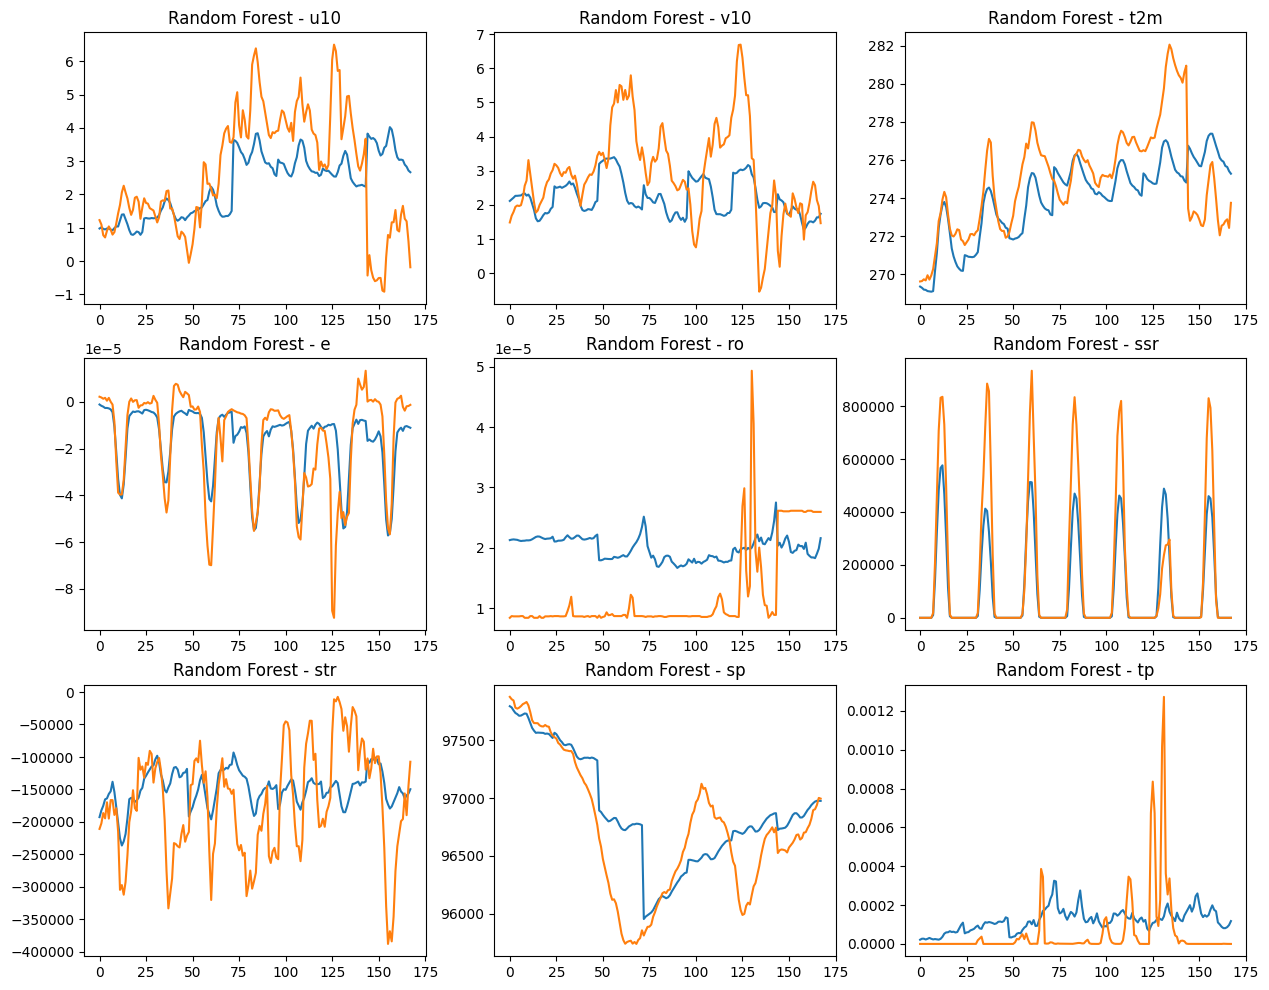
\includegraphics[width=\textwidth]{images/random_forest_week.png}
    \caption{Przebiegi czasowe dla algorytmu lasu losowego. Na żółto pokazane zostały dane 
    rzeczywiste, na niebiesko predykcje wygenerowane przez model}
    \label{forest-week}
\end{figure}

Kolejnym rozważanym modelem jest regresja logistyczna, która wydaje się najlepiej odzwierciedliła 
zachowania przebiegu temperatury, odparowania i promieniowania słonecznego. Większe wartości 
błędu dla tego modelu mogą być spowodowane gorszym dopasowaniem względem pozostałych parametrów, dla których
często prognozowane są nieprawidłowe wahania od rzeczywistego trendu.

\begin{figure}[H]
    \centering
    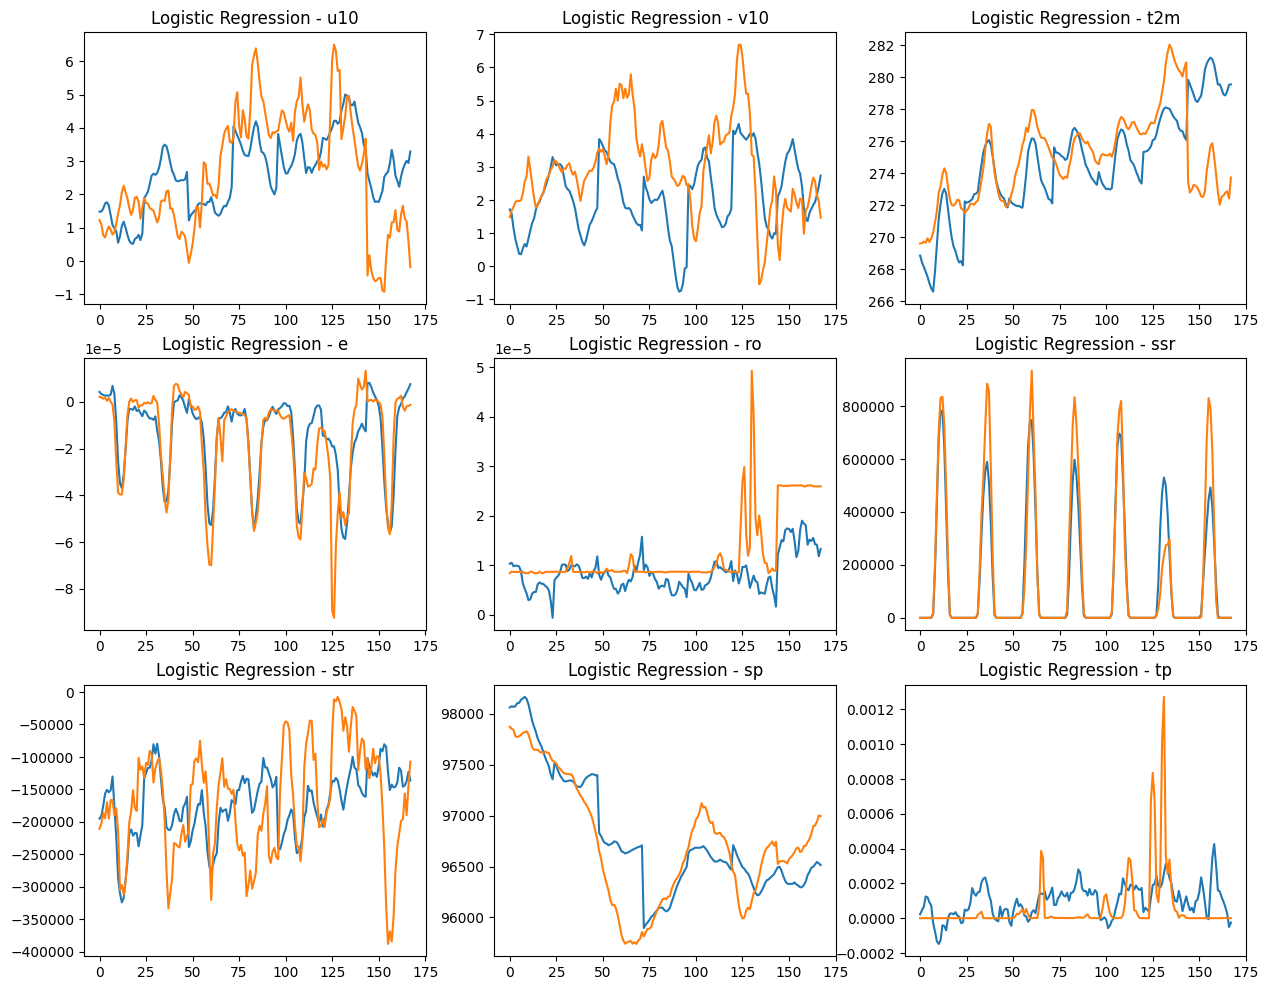
\includegraphics[width=\textwidth]{images/regression_week.png}
    \caption{Przebiegi czasowe dla algorytmu regresji logistycznej. Na żółto pokazane zostały dane 
    rzeczywiste, na niebiesko predykcje wygenerowane przez model}
    \label{regression-week}
\end{figure}

\begin{figure}[H]
    \centering
    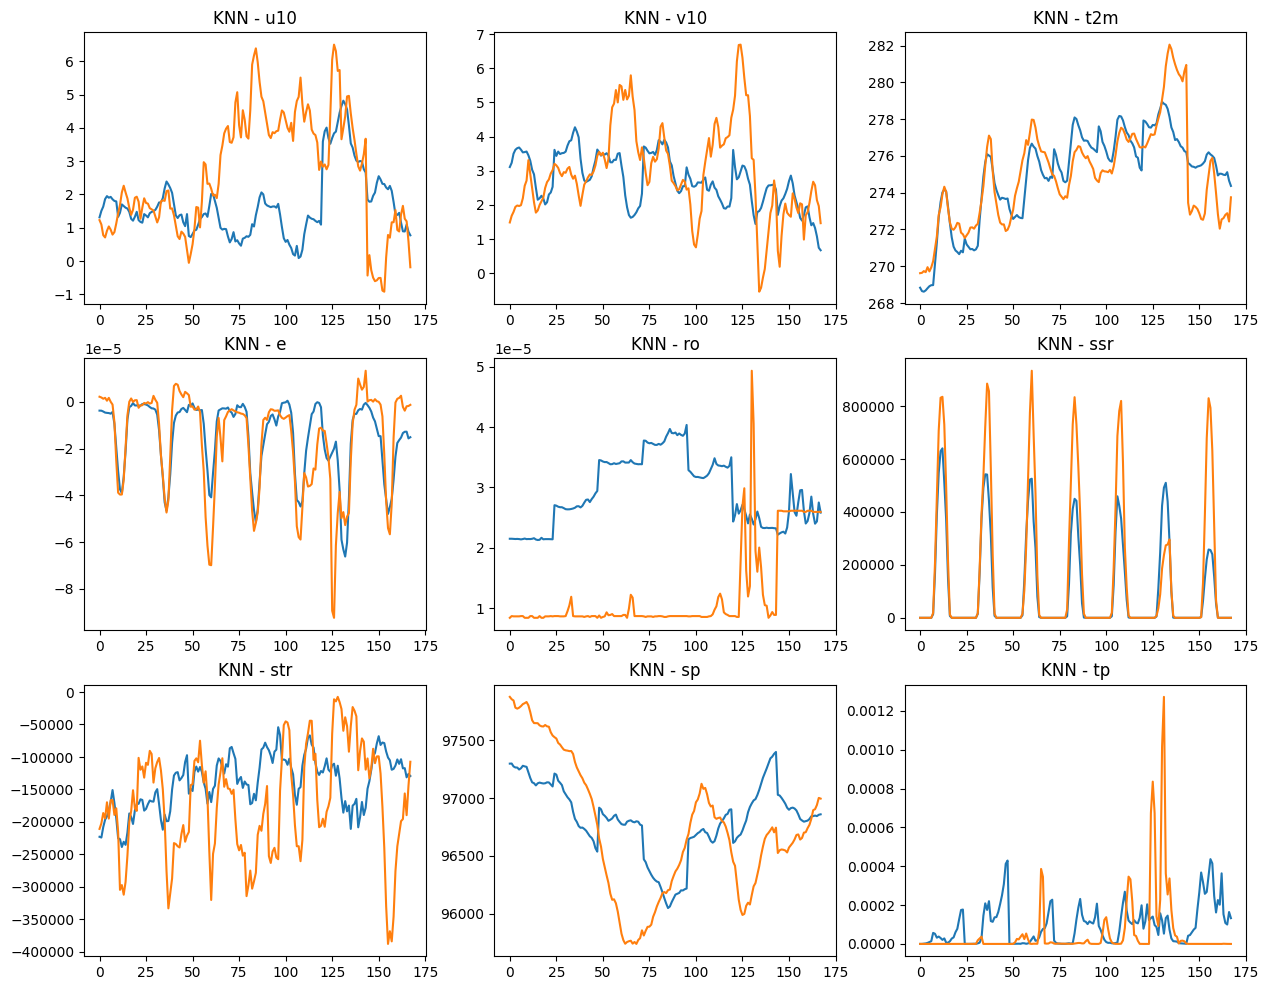
\includegraphics[width=\textwidth]{images/knn_week.png}
    \caption{Przebiegi czasowe dla algorytmu KNN. Na żółto pokazane zostały dane 
    rzeczywiste, na niebiesko predykcje wygenerowane przez model}
    \label{knn-week}
\end{figure}

Algorytm K najbliższych sąsiadów ma wyraźne trudności w rozpoznawaniu danych wejściowych różniących się od 
danych zawartych w zbiorze treningowym. Wyraźne odchylenia widoczne są przede wszystkim w przebiegach  
symbolizujących odpływ i ciśnienie atmosferyczne. Co więcej bardzo dużo opadów zostało fałszywie
zasygnalizowane. Model KNN okazuje się być niestosowny do problemu prognozowania pogody ze względu
na brak generalizacji nabytej wiedzy i dostosowania do nowych danych.

\pagebreak

Można także przeanalizować zdolność poszczególnych modeli do regresji względem poszczególnych atrybutów.
Tak na przykład na rysunku \ref{svr-mse-bar} pokazany został błąd średniokwadratowy dla modelu SVR, który był
jednym z modeli o najlepszych wynikach. Z przedstawionego wykresu wynika, że największy błąd jest generowany
przez prognozowanie promieniowania termicznego. Problemy w regresji względem tego atrybutu mogą być  
spowodowane między innymi jego wysoką wariancją i zależnością od procesów fizycznych nieujętych w zbiorze 
danych.

\begin{figure}[H]
    \centering
    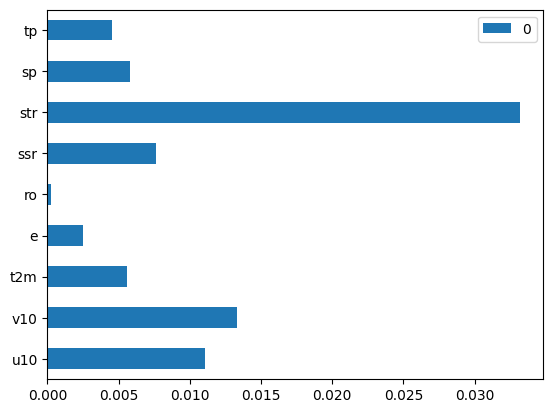
\includegraphics[width=\textwidth]{images/svr_mse_bar.png}
    \caption{Wartości błędu średniokwadratowego dla modelu SVR ze względu na poszczególne atrybuty danych.}
    \label{svr-mse-bar}
\end{figure}

Charakterystyka względem średniego błędu absolutnego wskazuje na te same wnioski. Najcięższymi parametrami
do przewidzenia były wartości promieniowania słonecznego oraz prędkości wiatru. Jednak nie wszystkie
parametry są jednakowo ujęte poprzez zastosowanie tej metryki. Stosując MAE widać, że błędy 
uwzględnione w prognozowaniu promieniowania słonecznego są mniejsze niż te wywołane przez ciśnienie
atmosferyczne oraz ilość opadów. Jest to przykład tego, jak używanie różnych metryk może prowadzić do 
odmiennych wniosków i być przyczyną odmiennej interpretacji.

\begin{figure}[H]
    \centering
    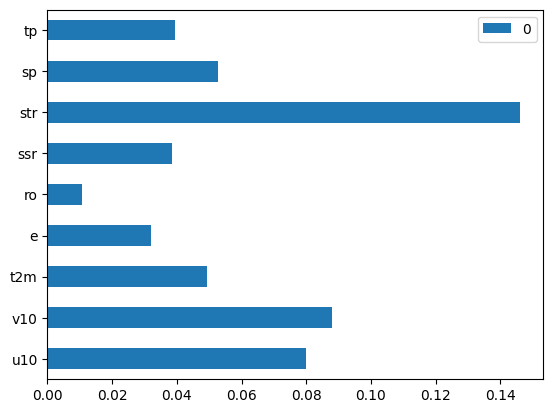
\includegraphics[width=\textwidth]{images/svr_mae_bar.png}
    \caption{Wartości średniego błędu absolutnego dla modelu SVR ze względu na poszczególne atrybuty danych.}
    \label{svr-mae-bar}
\end{figure}

Ponieważ MSE jest bardziej krytyczną metryką względem krótkotrwałych odchyleń o dużej różnicy względem
danych rzeczywistych, możemy wnosić, że różnice w danych generowanych dla wartości promieniowania słonecznego
mają charakter chwilowy, a po porównaniu wykresów szeregów czasowych widać, że największym problem okazuje
się prognozowanie wartości maksymalnej dla poszczególnych dni.

\pagebreak

% Inferential statistics: Report the results of any inferential 
% statistical analyses that you conducted to test your research 
% hypotheses, such as t-tests, ANOVA, regression analysis, or 
% other statistical tests. Be sure to include the statistical 
% significance of the results and the effect sizes.
\subsection{Analiza dystrybucji i korelacji}

W celach dalszej eksploracji otrzymanych wyników przeprowadzone zostało porównanie dystrybucji 
rzeczywistych parametrów atmosferycznych z predykcjami wygenerowanymi przez rozpatrywane algorytmy.
Na poniższym rysunku \ref{real-hist} zostały ponownie przedstawione histogramy dla oryginalnych danych pomiarowych.

\begin{figure}[H]
    \centering
    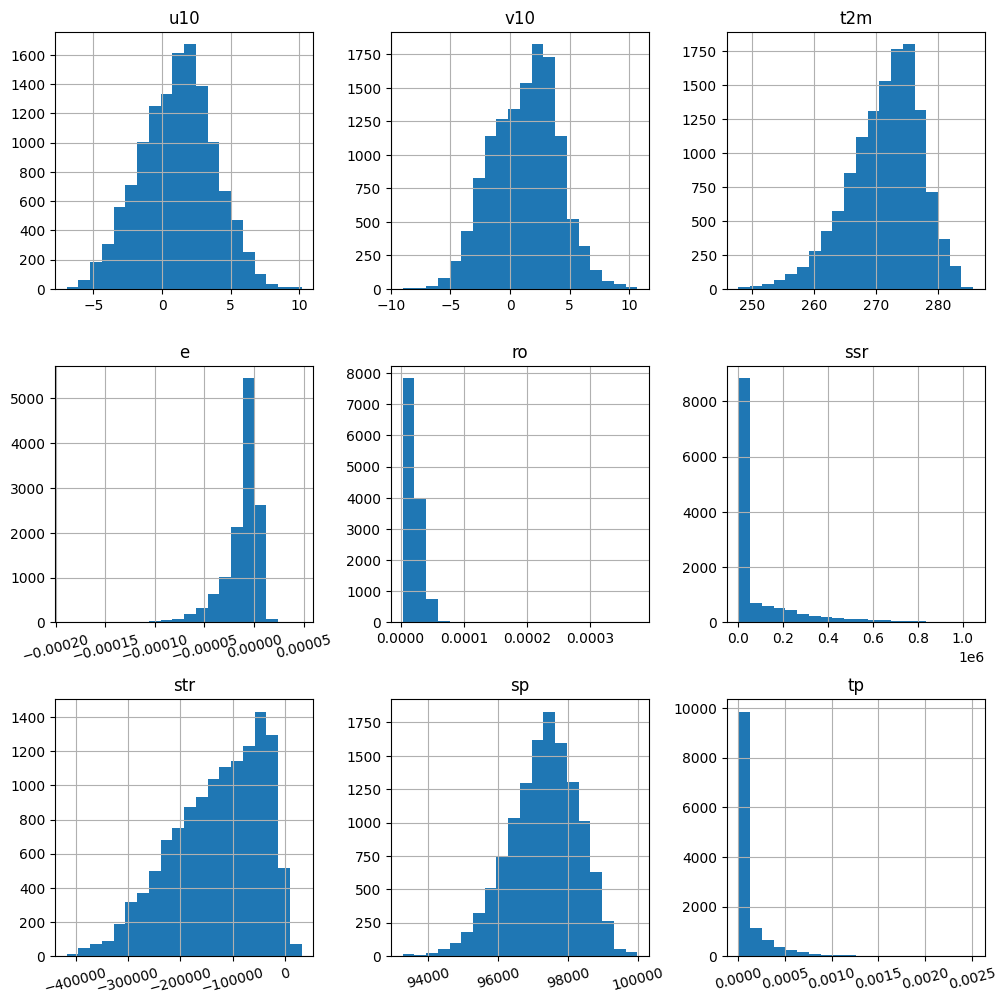
\includegraphics[width=\textwidth]{images/hist.png}
    \caption{Histogramy prezentujące dystrybucję danych rzeczywistych}
    \label{real-hist}
\end{figure}

Widzimy regularność w przedstawionych danych i choć nie wszystkie atrybuty podążają za dystrybucją normalną 
oraz występuje skośność w danych, to istnieje jednoznaczny model tworzący istniejące dane.

Nawet inspekcja najlepiej działającego algorytmu, którym jest SVR, pokazuje wady w utworzonych 
prognozach. Nieregularność dystrybucji danych szczególnie widoczna dla odpływów wody oraz
ciśnienia atmosferycznego ujawniają syntetyczne pochodzenie wygenerowanych predykcji. 
Co więcej, odparowanie, promieniowanie termiczne oraz ilość odpadów odbiegają od oryginalnego kształtu
dystrybucji danych.

\begin{figure}[H]
    \centering
    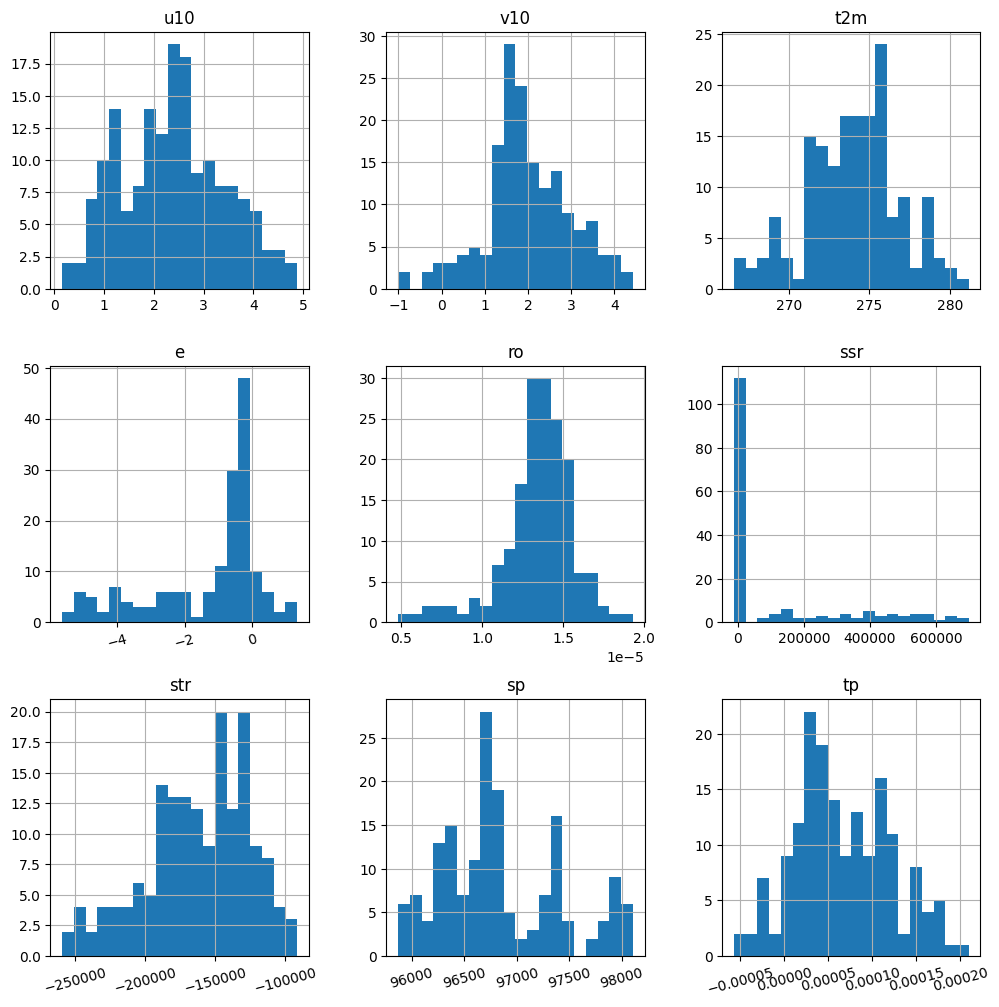
\includegraphics[width=\textwidth]{images/svr_hist.png}
    \caption{Histogramy prezentujące dystrybucję predykcji wygenerowanych przez algorytm SVR.}
    \label{svr-hist}
\end{figure}

\begin{figure}[H]
    \centering
    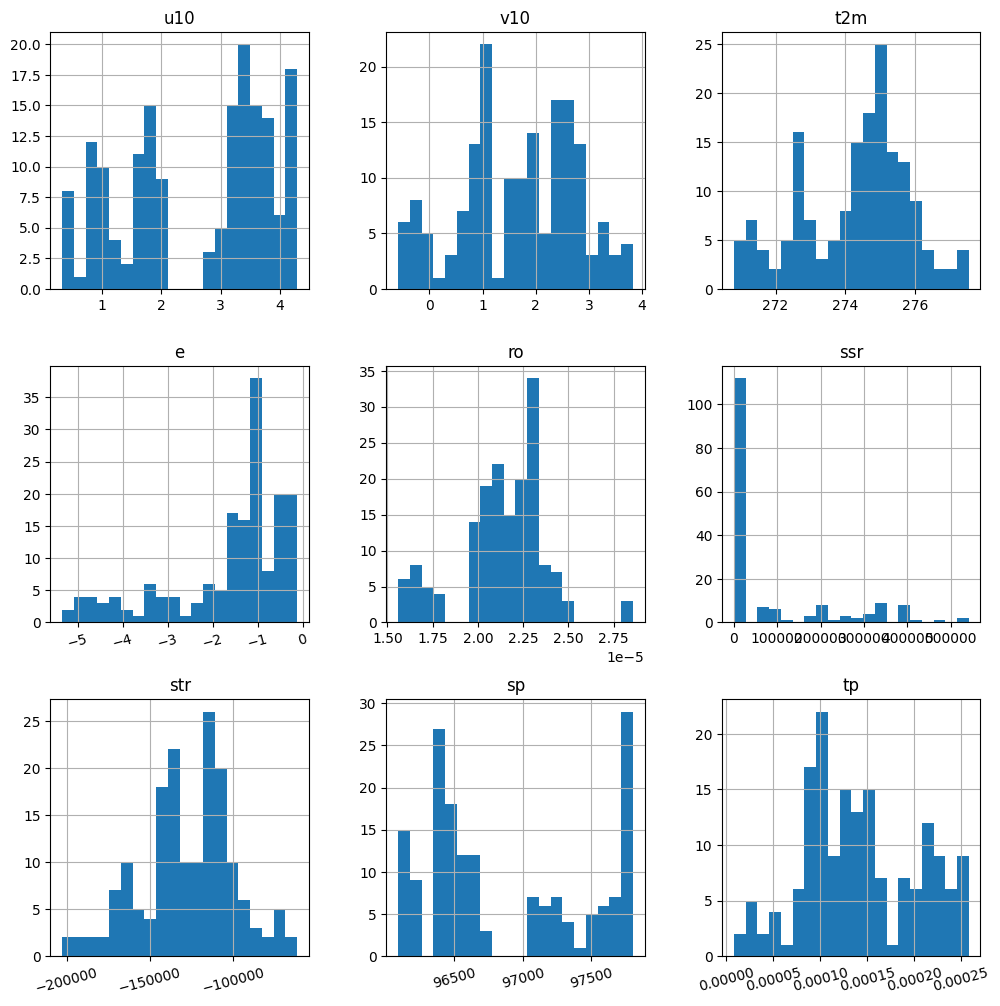
\includegraphics[width=\textwidth]{images/dt_hist.png}
    \caption{Histogramy prezentujące dystrybucję predykcji wygenerowanych przez algorytm drzewo decyzyjne.}
    \label{dt-hist}
\end{figure}

Na rysunku \ref{dt-hist} pokazane zostały analogiczne dystrybucje dla drzewa decyzyjnego. Luki w 
pewnych zakresach danych oraz brak ciągłości w dystrybucji ujawnia złe modelowanie zjawisk atmosferycznych,
poprzez nieprawidłowe odwzorowanie danych rzeczywistych. 

\begin{figure}[H]
    \centering
    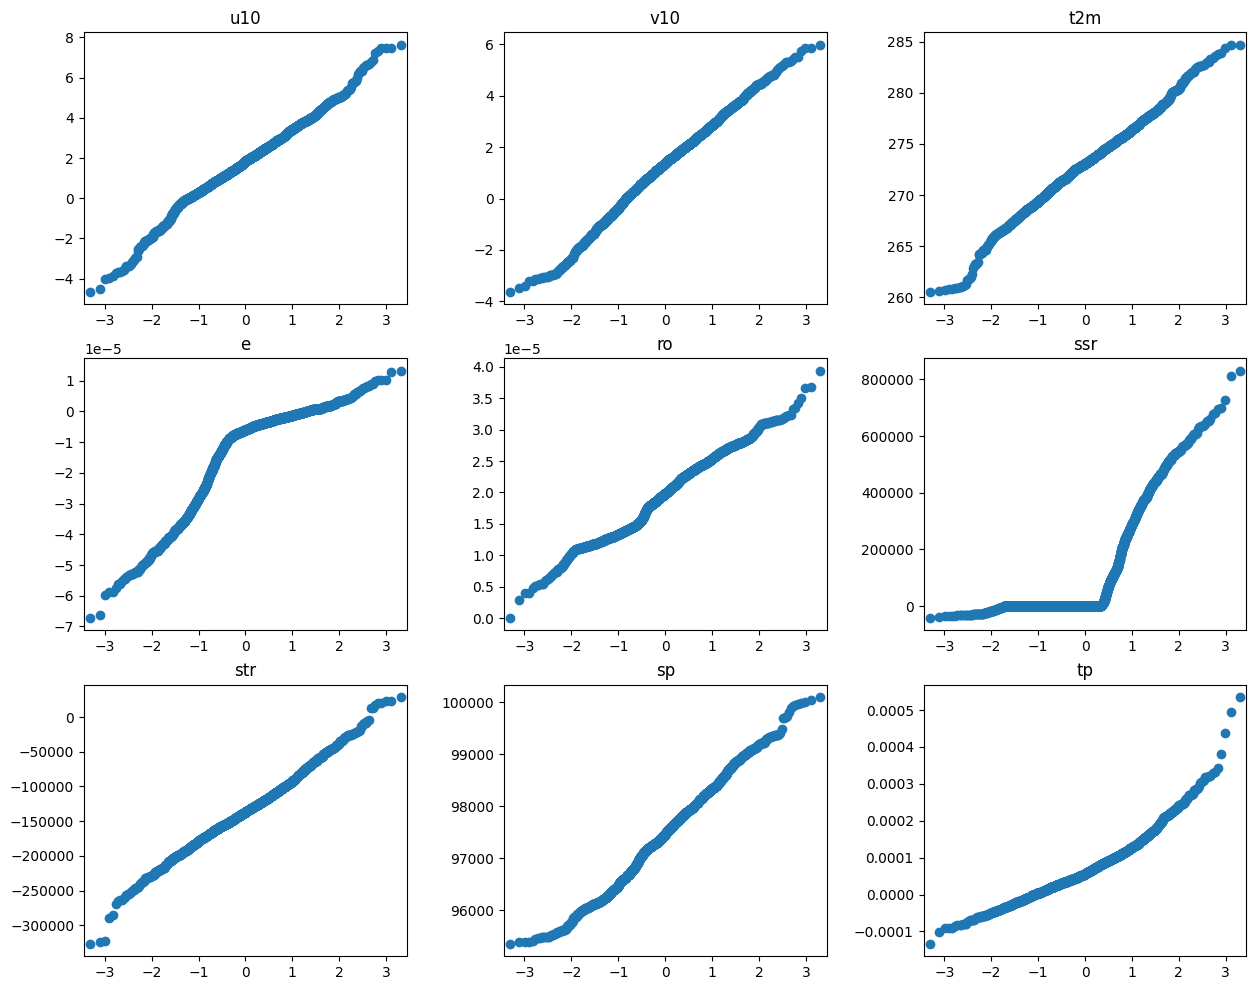
\includegraphics[width=\textwidth]{images/svr_qq.png}
    \caption{Wykresy QQ stworzone dla modelu SVR}
    \label{svr-qq}
\end{figure}

Aby przeprowadzić dalszą analizę, stworzone zostały wykresy QQ pokazane na rysunku \ref{svr-qq} oraz \ref{dt-qq}.
W przypadku algorytmu SVR większość danych podąża za dystrybucją normalną, nawet w przypadkach,
gdy dla danych rzeczywistych nie było to prawdą. Wyjątkiem od tego są odparowanie oraz promieniowanie 
termiczne, które odbiegają od ogólnego trendu i zdają się sumą dwóch dystrybucji normalnych.

Analogiczny wykres dla drzewa decyzyjnego pokazuje chaotyczność w wytworzonych danych, jeszcze raz 
udowadniając niestosowność zastosowanego algorytmu. Poprzez użycie drzewa decyzyjnego reprodukcja
rzeczywistych parametrów jest niemożliwa, a utworzone prognozy pogodowe odbiegają od oczekiwanych wartości.

\begin{figure}[H]
    \centering
    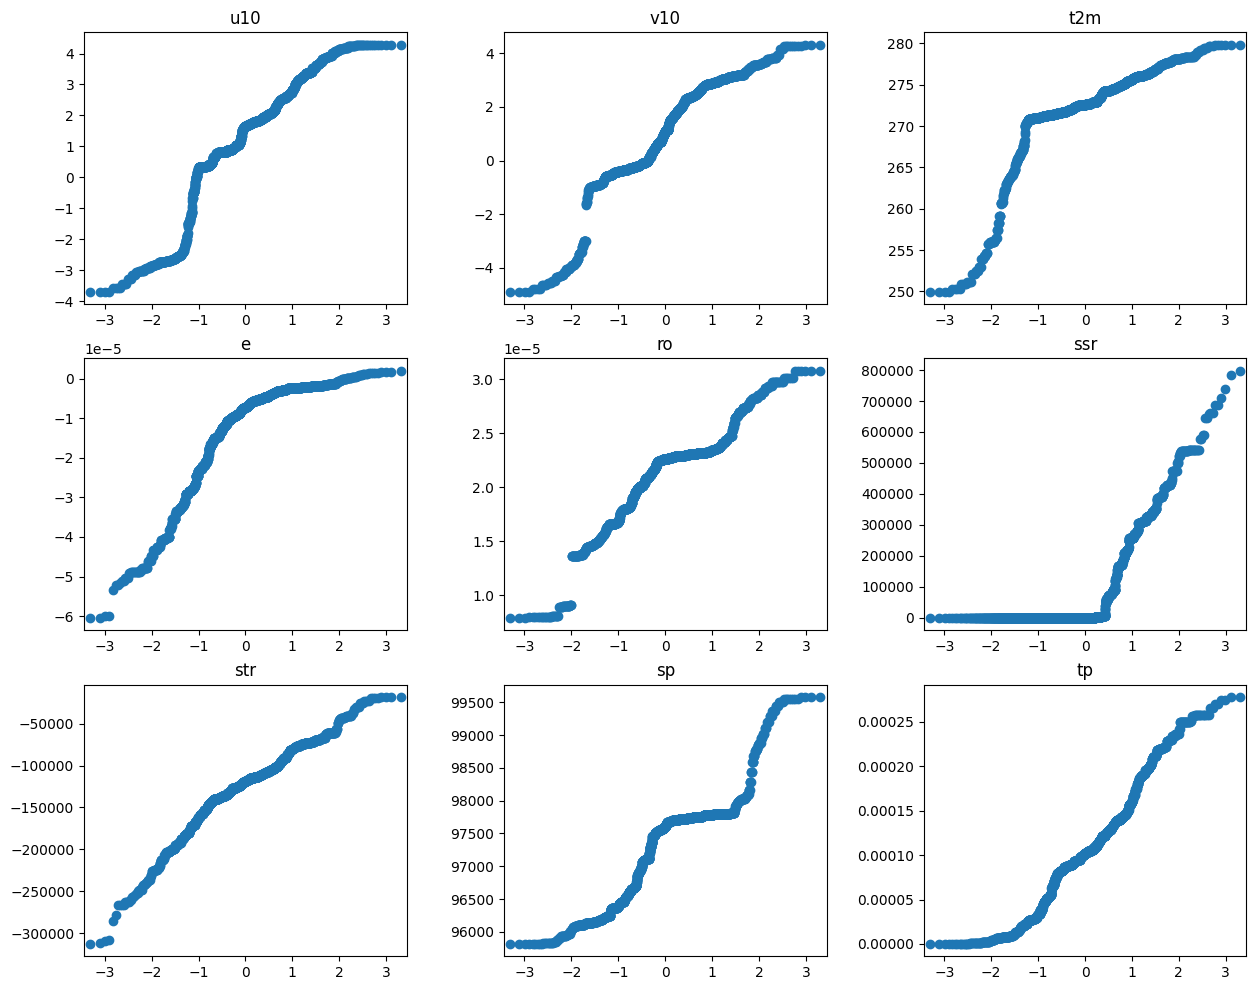
\includegraphics[width=\textwidth]{images/dt_qq.png}
    \caption{Wykresy QQ stworzone dla modelu drzewa decyzyjnego}
    \label{dt-qq}
\end{figure}

Kolejnym pokazanym rysunkiem są wykresy pudełkowe dla algorytmu SVR pokazane na zdjęciu \ref{svr-box}. 
Widzimy na nich o wiele mniejszą ilość
danych odstających w stosunku do tych samych wykresów wygenerowanych dla danych rzeczywistych. Co więcej,
większość parametrów zdaje się posiadać symetryczny rozkład, co nie było prawdą dla modelowanych danych.

\begin{figure}[H]
    \centering
    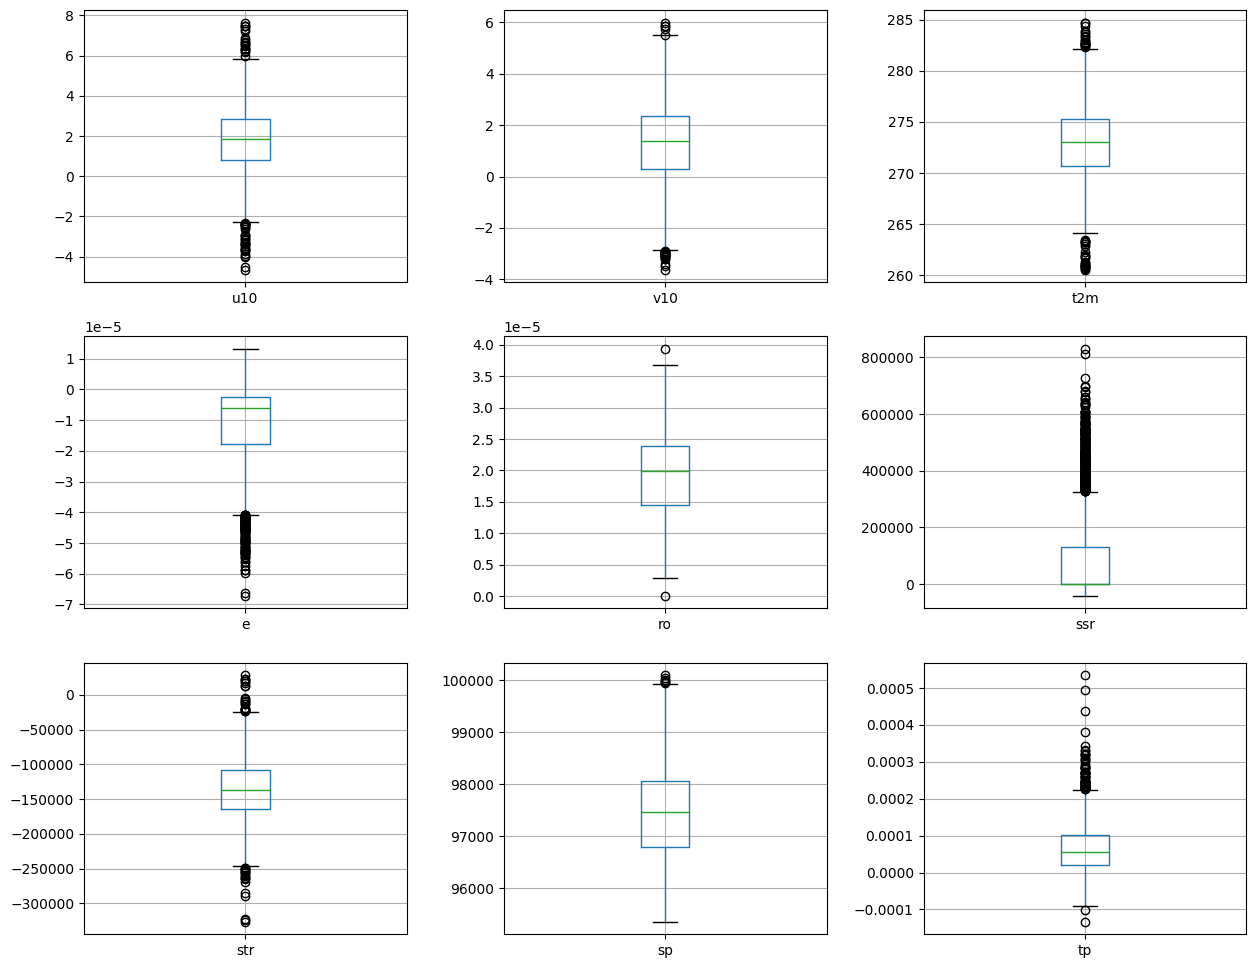
\includegraphics[width=.8\textwidth]{images/svr_box.png}
    \caption{Wykresy pudełkowe dla modelu SVR}
    \label{svr-box}
\end{figure}

\begin{figure}[H]
    \centering
    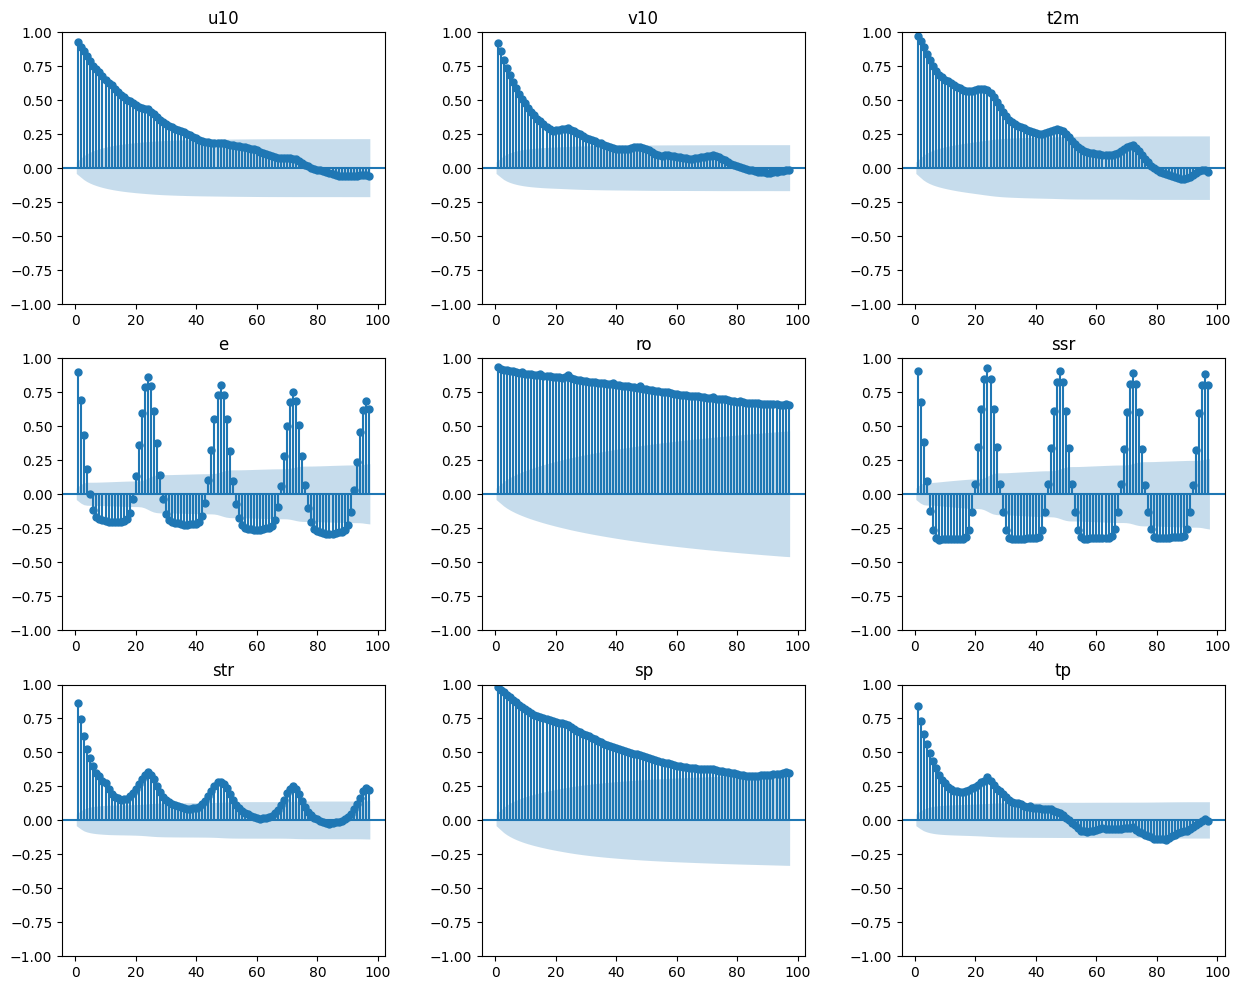
\includegraphics[width=.8\textwidth]{images/svr_autocorr.png}
    \caption{Współczynnik autokorelacji dla SVR dla wartości przesunięcia w zakresie czterech dni}
    \label{svr-autocorr}
\end{figure}

Obserwując wykresy autokorelacji, możemy także zaobserwować zależności, które nie występowały pierwotnie w 
zbiorze danych. Pierwotnie szeregi czasowe dla prędkości wiatru nie ujawniały natury cyklicznej, jednak 
na wykresie \ref{svr-autocorr} widać periodyczne skoki w wartości autokorelacji następujące co jeden dzień.
Ten sam wniosek może zostać wyciągnięty względem ilości opadów, które dla analizowanego zbioru danych 
ujawniały jednostajnie spadającą autokorelację, a w tym przypadku widzimy nieregularny przebieg z okresowymi
skokami. Mimo to wartości dla reszty atrybutów są bardzo bliskie względem symulowanych danych.

\begin{figure}[H]
    \centering
    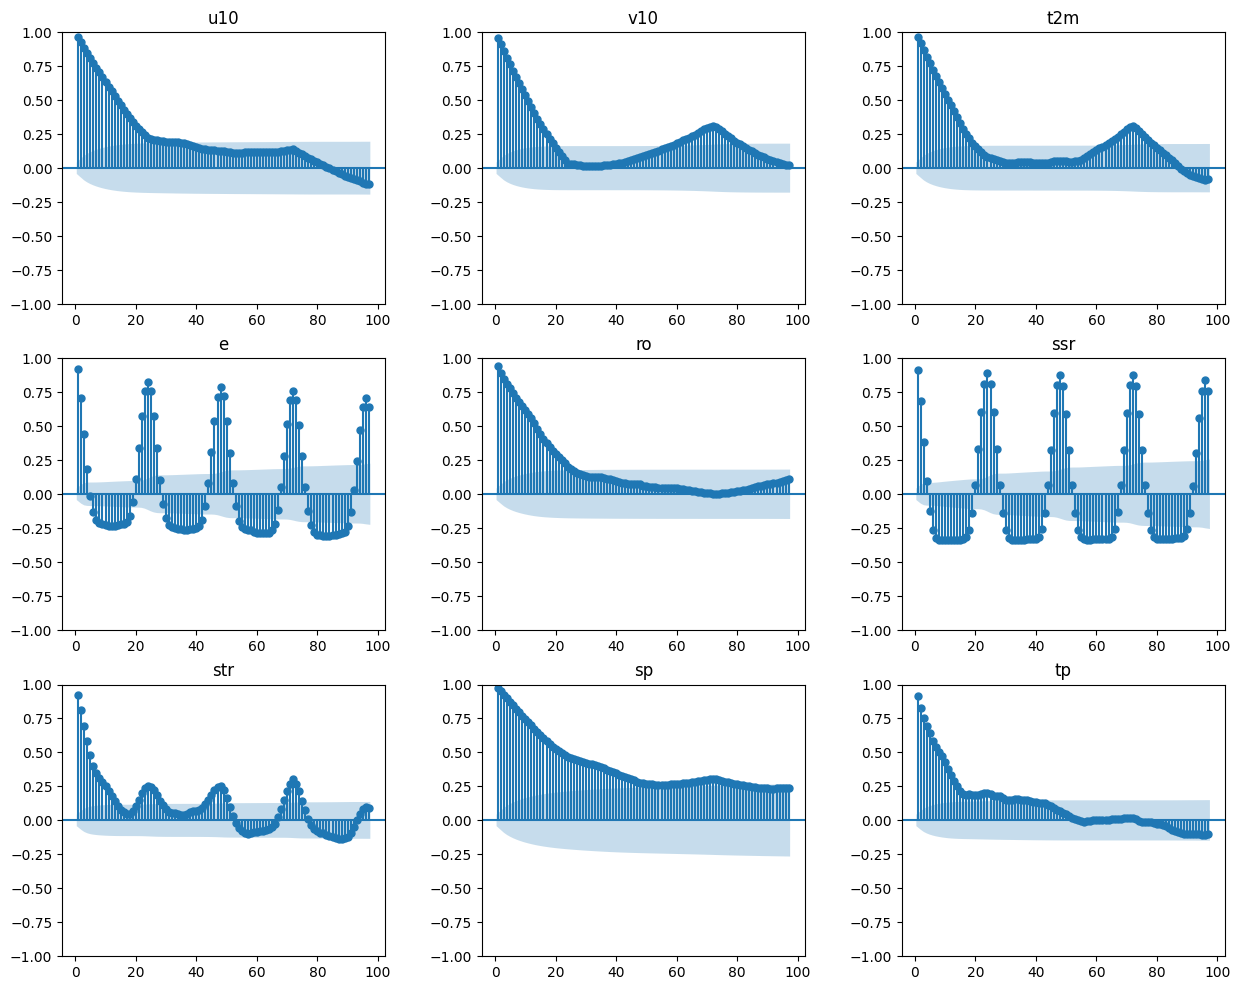
\includegraphics[width=\textwidth]{images/dt_autocorr.png}
    \caption{Współczynnik autokorelacji dla drzewa decyzyjnego dla wartości przesunięcia w zakresie czterech dni}
    \label{dt-autocorr}
\end{figure}

W przypadku drzewa decyzyjnego, dla którego autokorelacja została ukazana na wykresie \ref{dt-autocorr},
wygenerowane wykresy pokazują o wiele bardziej losową naturę. Nagłe skoki nie podążają za dziennymi cyklami,
co może wskazywać na "ślepe" powtarzanie wcześniej zaobserwowanych pomiarów. 

\begin{figure}[H]
    \centering
    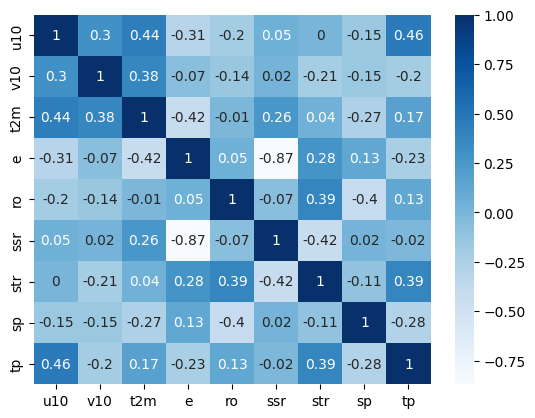
\includegraphics[width=\textwidth]{images/svr_corr_matrix.png}
    \caption{Korelacja pomiędzy parametrami w stworzonych prognozach dla algorytmu SVR}
    \label{svr-corr-matrix}
\end{figure}

Na powyższym rysunku \ref{svr-corr-matrix} pokazana została korelacja pomiędzy poszczególnymi atrybutami.
Pokazane wartości są bliskie w wartości do podobnej analizy przeprowadzonej dla danych pomiarowych. 
Największa korelacja istnieje pomiędzy promieniowaniem słonecznym a odparowaniem i wynosi -0,87 (-0,63 dla
rzeczywistego zbioru). Poza tym brak bardziej znaczących wartości z pominięciem tp-str, str-ssr i temperaturą
względem prędkości wiatru. Jednym z odchyleń względem rzeczywistości zdaje się wysoka wartość dla 
relacji między ciśnieniem atmosferycznym a odpływem cieków wodnych, która nie występuję w naturze.

\begin{figure}[H]
    \centering
    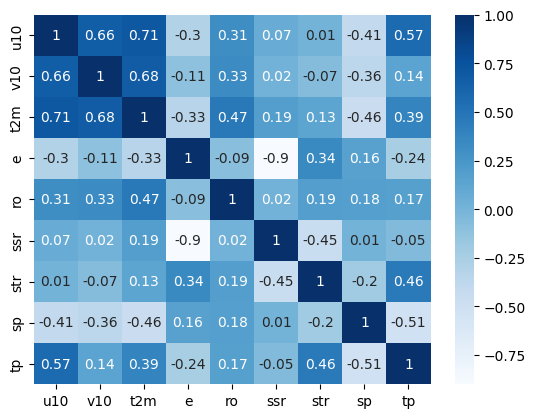
\includegraphics[width=\textwidth]{images/dt_corr_matrix.png}
    \caption{Korelacja pomiędzy parametrami w stworzonych prognozach dla drzewa decyzyjnego}
    \label{dt-corr-matrix}
\end{figure}

Taki sam wykres został stworzony dla drzewa decyzyjnego na rysunku \ref{dt-corr-matrix}. Możemy na nim 
zaobserwować podobne wzorce, lecz z o wiele większą korelacją pomiędzy poszczególnymi atrybutami. 
Wartości korelacji sięgają wartości od -0,9 aż do 0,71. Algorytm drzewa decyzyjnego zdaje się 
bazować swoje wyniki bezpośrednio na relacjach występujących pomiędzy pojedynczymi atrybutami,
a w rezultacie ignorując głębsze zależności występujące w danych.


% Tables and figures: Present your data in tables and figures 
% that are clear, concise, and easy to read. Ensure that your 
% tables and figures are properly labeled and that they effectively 
% illustrate your findings.

% Subgroup analyses: Conduct subgroup analyses if relevant to 
% your research questions. For example, if you are comparing the 
% performance of different machine learning models, you might conduct 
% subgroup analyses based on the type of model used or the size of the training data.
\subsection{Porównanie modeli}

\begin{figure}[H]
    \centering
    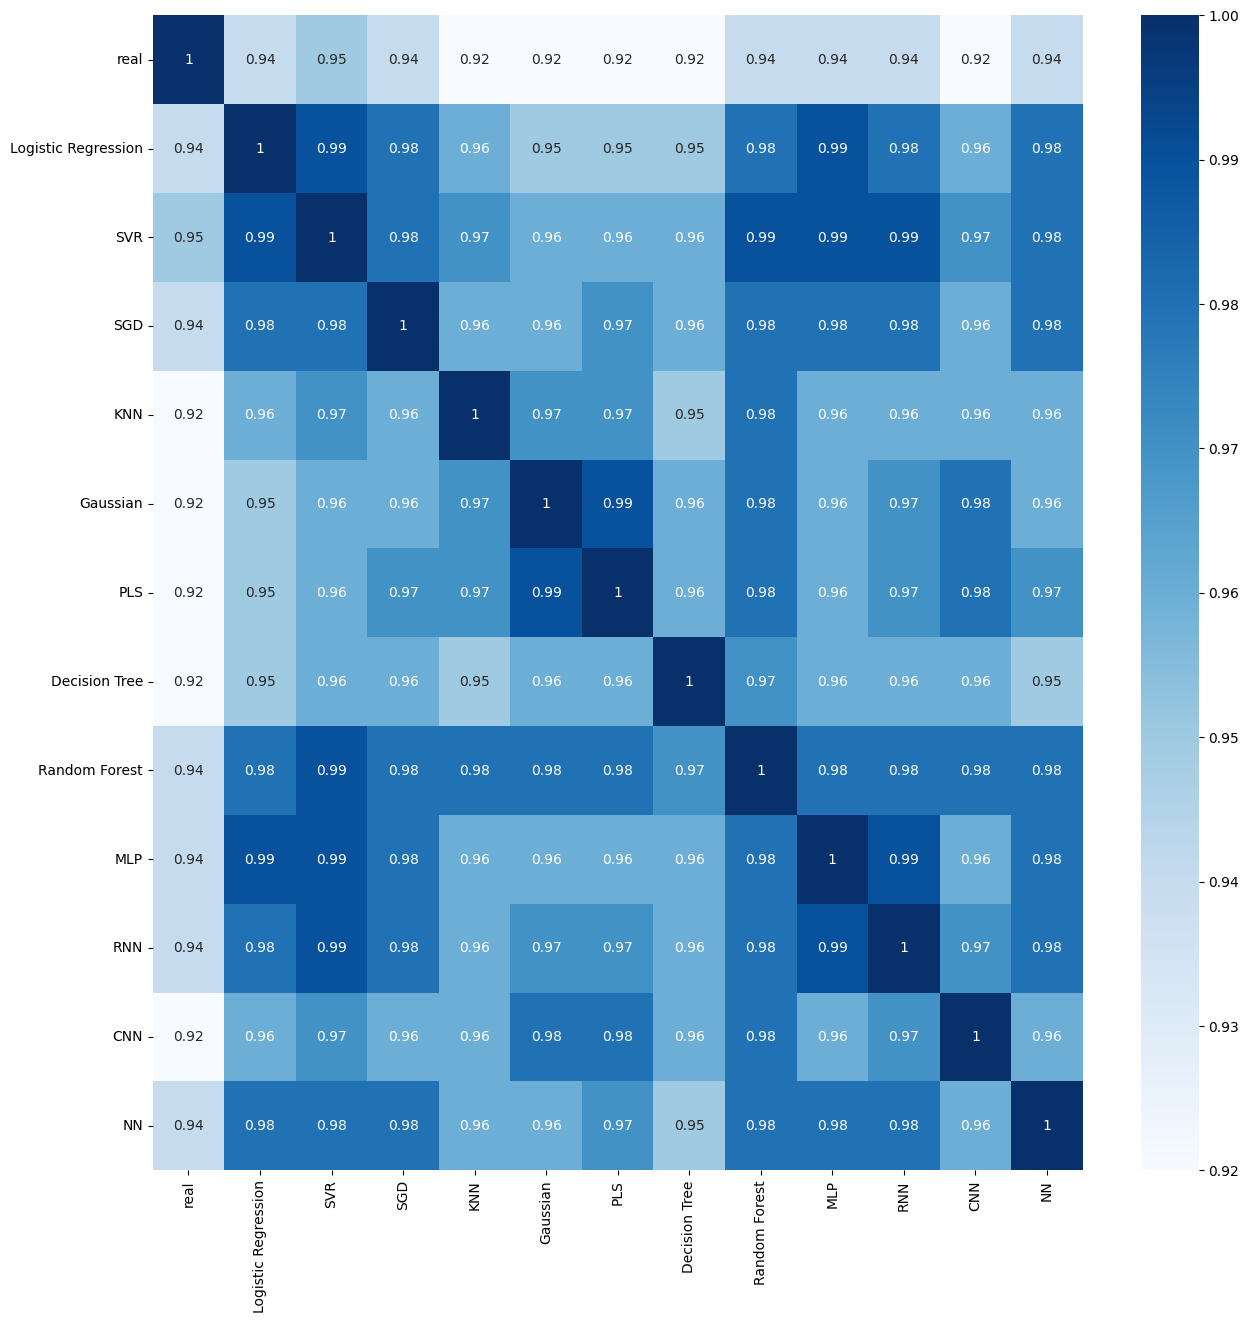
\includegraphics[width=\textwidth]{images/pred_corr.png}
    \caption{Korelacja pomiędzy wynikami stworzonymi poprzez poszczególne modele}
    \label{pred_corr}
\end{figure}

Porównując modele, można zastosować te same metryki jak w przypadku ewaluacji predykcji względem 
danych rzeczywistych. Największe wartości korelacji są widoczne pomiędzy modelami SVR, regresji logistycznej,
lasu losowego, MLP i RNN. Są to wszystkie modele, które w przeprowadzonych eksperymentach uzyskały najlepsze
rezultaty. Kolejną grupą algorytmów znajdujących się blisko siebie jest regresja gaussowska, PLS oraz CNN,
które, chociaż nie uzyskały najlepszych rezultatów, znajdowały się wśród algorytmów o średniej wydajności.
Drzewo decyzyjne będące przykładem najgorszego z rozważanych algorytmów znajduję się w dużej odległości
od pozostałych modeli.

Podobną analizę można przeprowadzić również ze względu na wartość błędu absolutnego i średniokwadratowego,
czego wyniki zostały zobrazowane na rysunku \ref{mse-matrix} oraz \ref{mae-matrix}.

\begin{figure}[H]
    \centering
    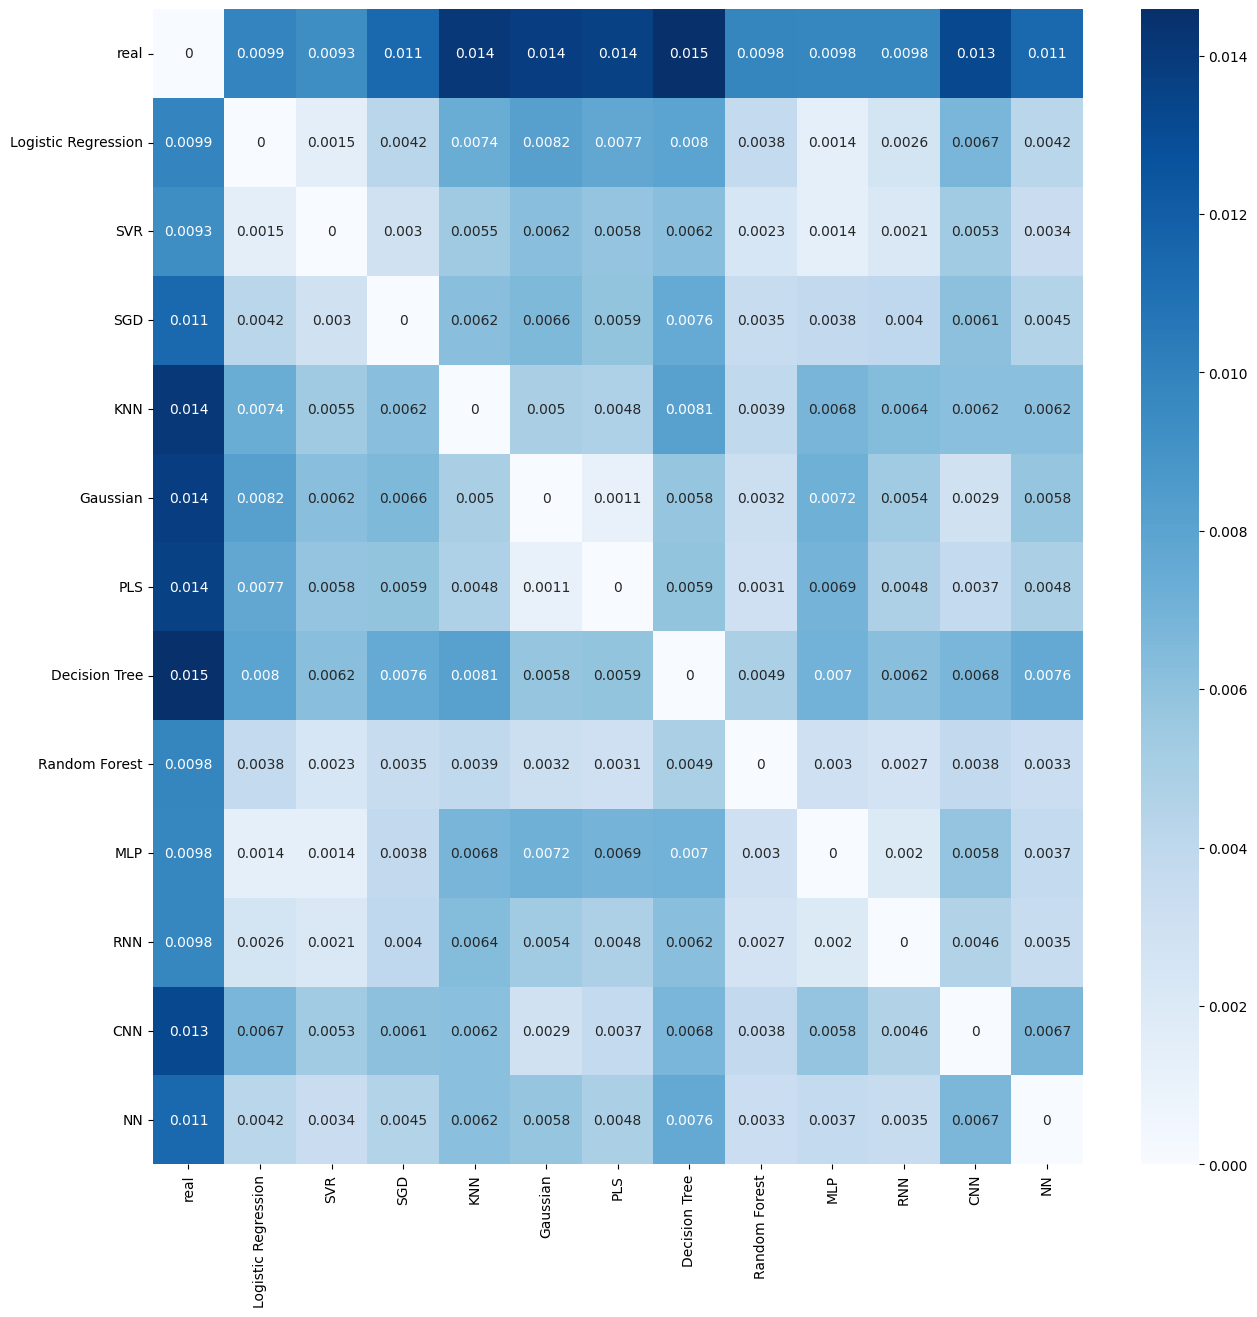
\includegraphics[width=\textwidth]{images/mse_matrix.png}
    \caption{Wartość błędu średniokwadratowego pomiędzy wynikami stworzonymi poprzez poszczególne modele}
    \label{mse-matrix}
\end{figure}

\begin{figure}[H]
    \centering
    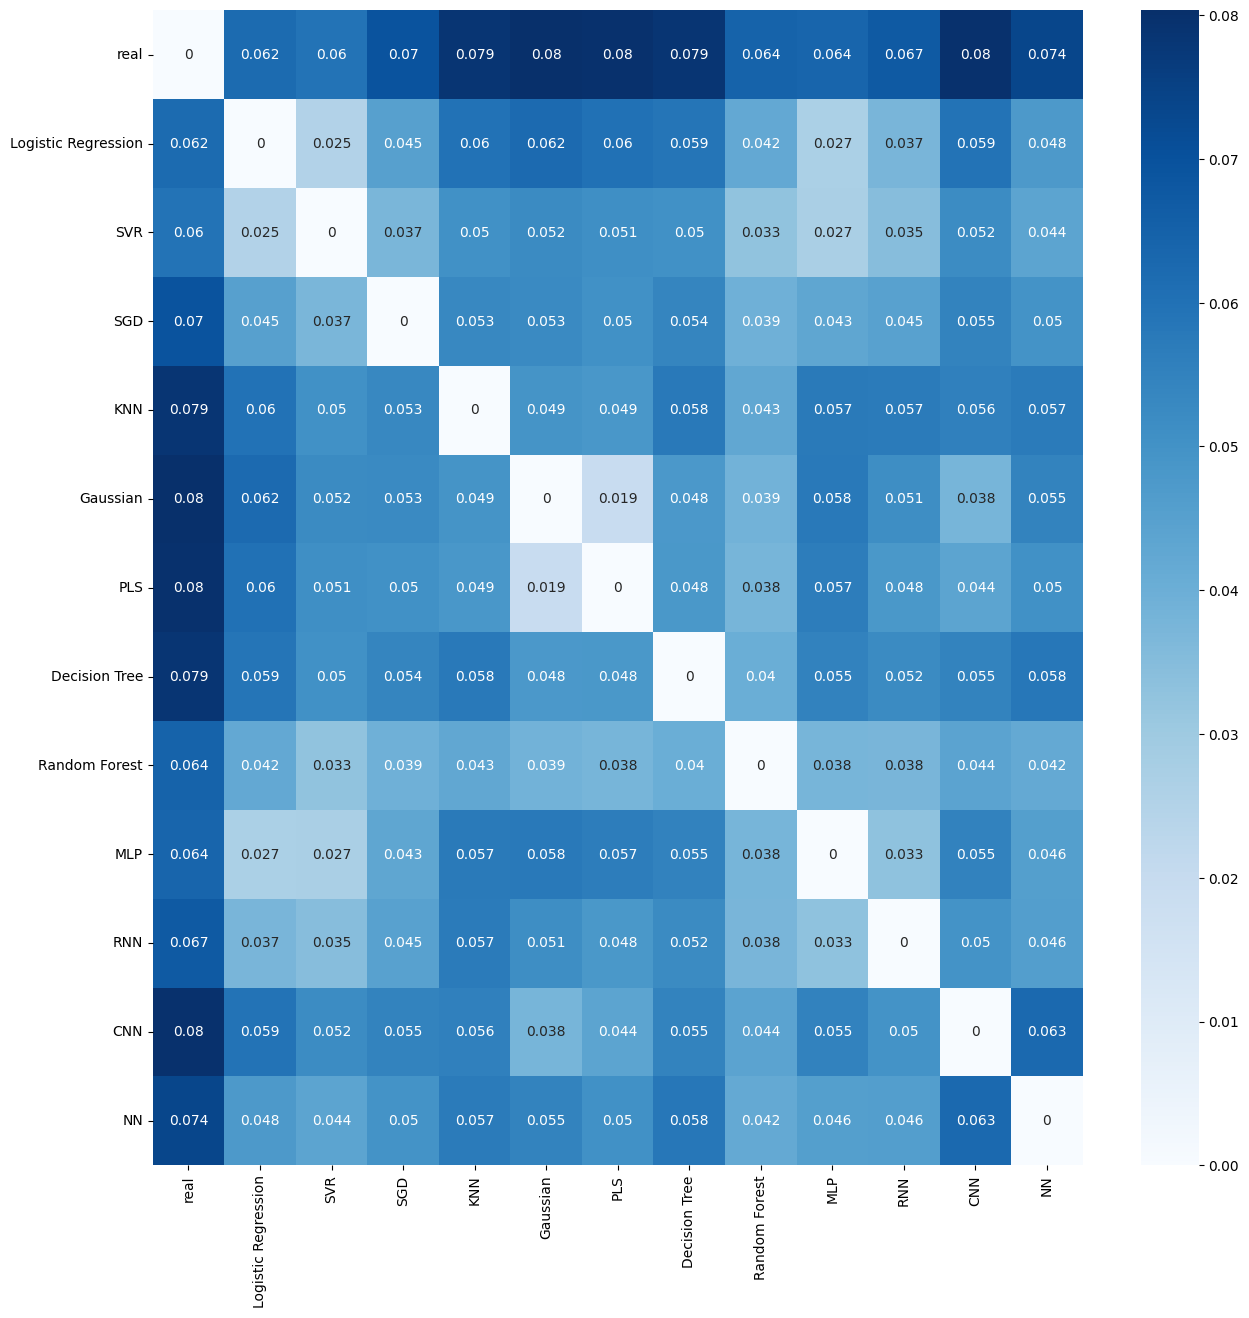
\includegraphics[width=\textwidth]{images/mae_matrix.png}
    \caption{Wartość średniego błędu absolutnego pomiędzy wynikami stworzonymi poprzez poszczególne modele}
    \label{mae-matrix}
\end{figure}

Wszystkie metryki wskazują na podobne rozdysponowanie rozważanych modeli względem siebie. Warto również wskazać
fakt, że wartość błędu większości modeli względem siebie nie przekraczała wartości błędu względem wartości
referencyjnych.

% \begin{figure}[H]
%     \centering
%     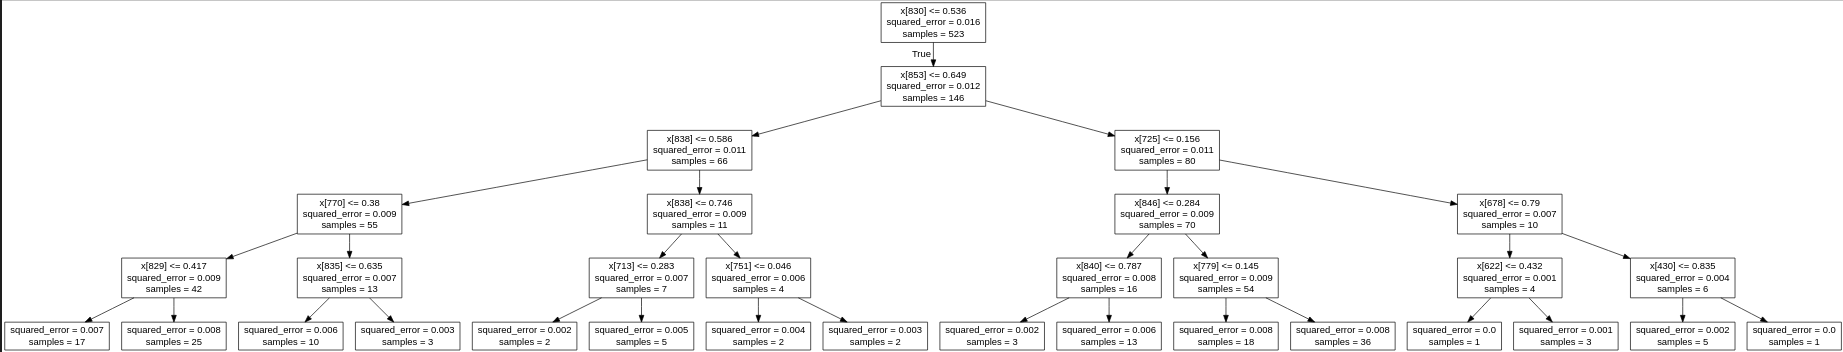
\includegraphics[width=\textwidth]{images/tree.png}
%     \caption{}
%     \label{tree-graph}
% \end{figure}

% Interpretation: Provide an interpretation of your findings and 
% relate them back to your research questions or hypotheses. Discuss 
% the implications of your results for the broader field of weather 
% prediction and the use of artificial intelligence and machine learning 
% techniques in this area.
\subsection{Interpretacja}

% Limitations: Discuss any limitations of your study that may 
% have affected the validity or generalizability of your findings. 
% Be sure to acknowledge any potential sources of bias or confounding variables.
\subsection{Ograniczenia}